% !TeX spellcheck = en_US
%\documentclass[11pt,a4paper]{article}
\documentclass[11pt
  , a4paper
  , article
  , oneside
%  , twoside
%  , draft
]{memoir}

\usepackage{control}
\usepackage[numbers]{natbib}


\begin{document}

\newcommand{\technumber}{
  RAON Control-Document Series\\
  Revision : v1.0,   Release : 2015-03-16 fixed date}
\title{\textbf{FPGA - Zynq}}

\author{이상일\thanks{silee7103@ibs.re.kr}, 손창욱 \\

  Rare Isotope Science Project\\
  Institute for Basic Science, Daejeon, South Korea
}
\date{\today}

\renewcommand{\maketitlehooka}{\begin{flushright}\textsf{\technumber}\end{flushright}}
%\renewcommand{\maketitlehookb}{\centering\textsf{\subtitle}}
%\renewcommand{\maketitlehookc}{C}
%\renewcommand{\maketitlehookd}{D}

\maketitle

\begin{abstract}
RAON is a particle accelerator to research the interaction between the nucleus forming a rare isotope as Korean heavy-ion accelerator. RAON accelerator consists of a number of facilities and equipments as a large-scaled experimental device operating under the distributed environment. For synchronization control between these experimental devices, timing system of the RAON uses the VME-based EVG/EVR system. This paper is intended to test high-speed device control with timing event signal. To test the high-speed performance of the control logic with the minimized event signal delay, we are planing to establish the step motor controller testbed applying the FPGA chip. The testbed controller will be configured with Zynq 7000 series of Xilinx FPGA chip. Zynq as SoC (System on Chip) is divided into PS (Processing System) with PL (Programmable Logic). PS with the dual-core ARM cpu is performing the high-level control logic at run-time on linux operating system. PL with the low-level FPGA I/O signal interfaces with the step motor controller directly with the event signal received from timing system.

This paper describes the content and performance evaluation obtaining from the step motor control through the various synchronized event signal received from the timing system.

\end{abstract}

\clearpage

FPGA(Field Programmable Gate Array)는 Hardware의 IC 소자의 gate array를 사용자가 program하여 회로를 구성할 수 있는 chip을 말한다. FPGA 프로그램 개발은 HDL(Hardware Description Language) 개발표준 언어를 사용하며 프로그램 할 수 있으며 아래와 같은 두 가지 HDL 언어를 지원한다.

\begin{itemize}
	\item VHDL
	\item Verilog HDL
\end{itemize}

본 문서에는 Xilinx의 FPGA Chip 중 Zynq 사용을 위한 내용을 기술한다. Zynq의 특징은 앞서 설명한 FPGA의 특징과 ARM CPU를 내장한 embedded 특징 모두 가지는 하나의 SoC(System on Chip) 이다.  따라서 Zynq Chip에는 기존 FPGA에 가지는 장점에 embedded 형태의 운영체제를 가질 수 있는 장점이 있다. 또한 이 둘간의 interface는 AXI Bus interface를 통한 메모리 맵을 통하여 데이터 통신이 가능하다. 따라서 고속 신호처리를 위하여는 FPGA I/O를 low level(hardware) 단에서 처리를 하며, 상위 레벨과의 인터페이스 및 주요 제어로직은 CPU 모듈에서 처리 할 수 있는 설계가 가능하다. 이는 가속기 제어 operation sequence에 따른 timing event의 external trigger를 입력으로 받아 고속의 신호를 처리하여야 하는 application에 활용 할 수 있다. 또한 MPS(Machine Protection System)와 같은 고속의 application에 적용할 수 있으리라 판단된다.
Zynq는 ARM 계열의 CPU를 가지고 있으며 여기에 linux 운영체제를 쉽게 올릴 수 있는 petalinux softeware tool을 제공한다. 

\begin{figure}[h!]
	\centering
	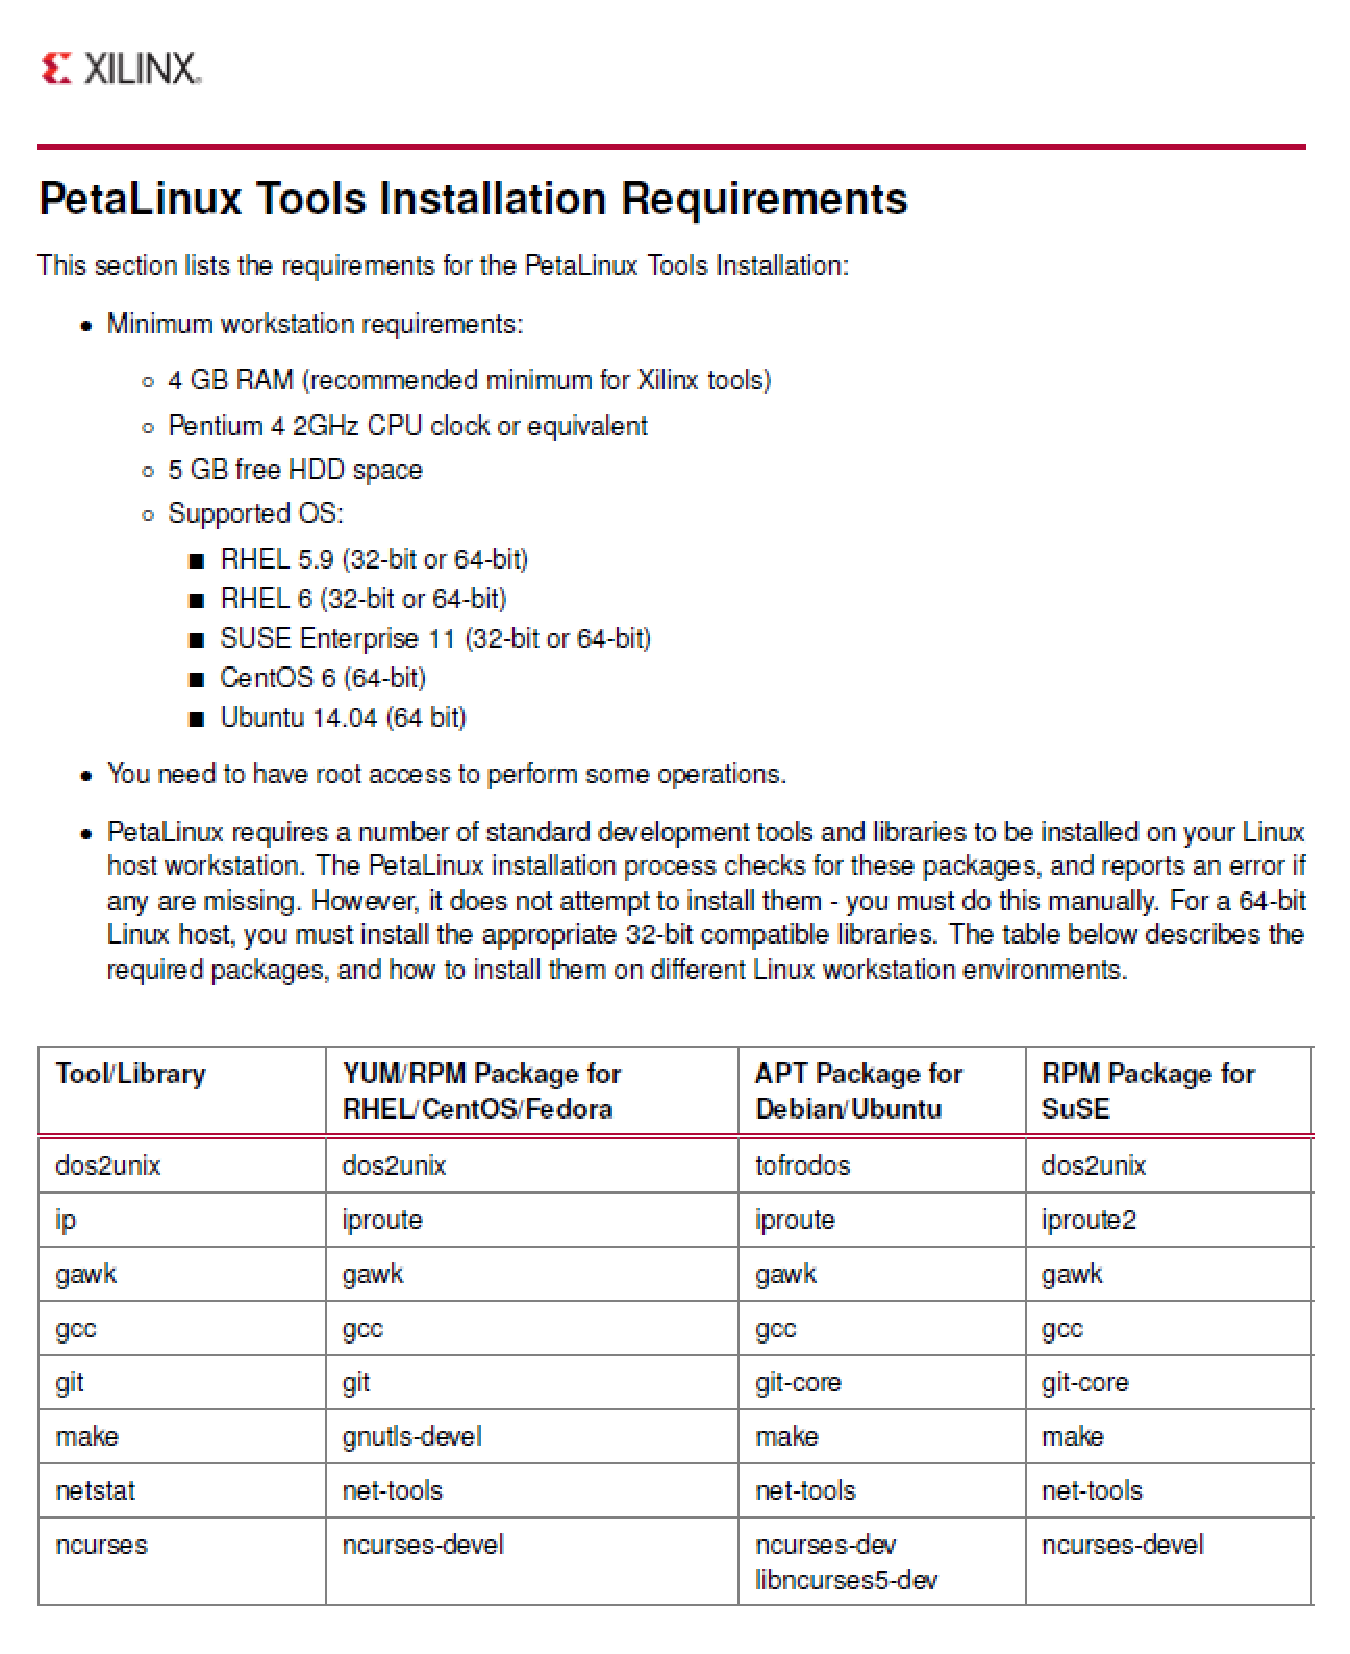
\includegraphics[width=0.85\textwidth]{./images/preinstall_2.eps}
	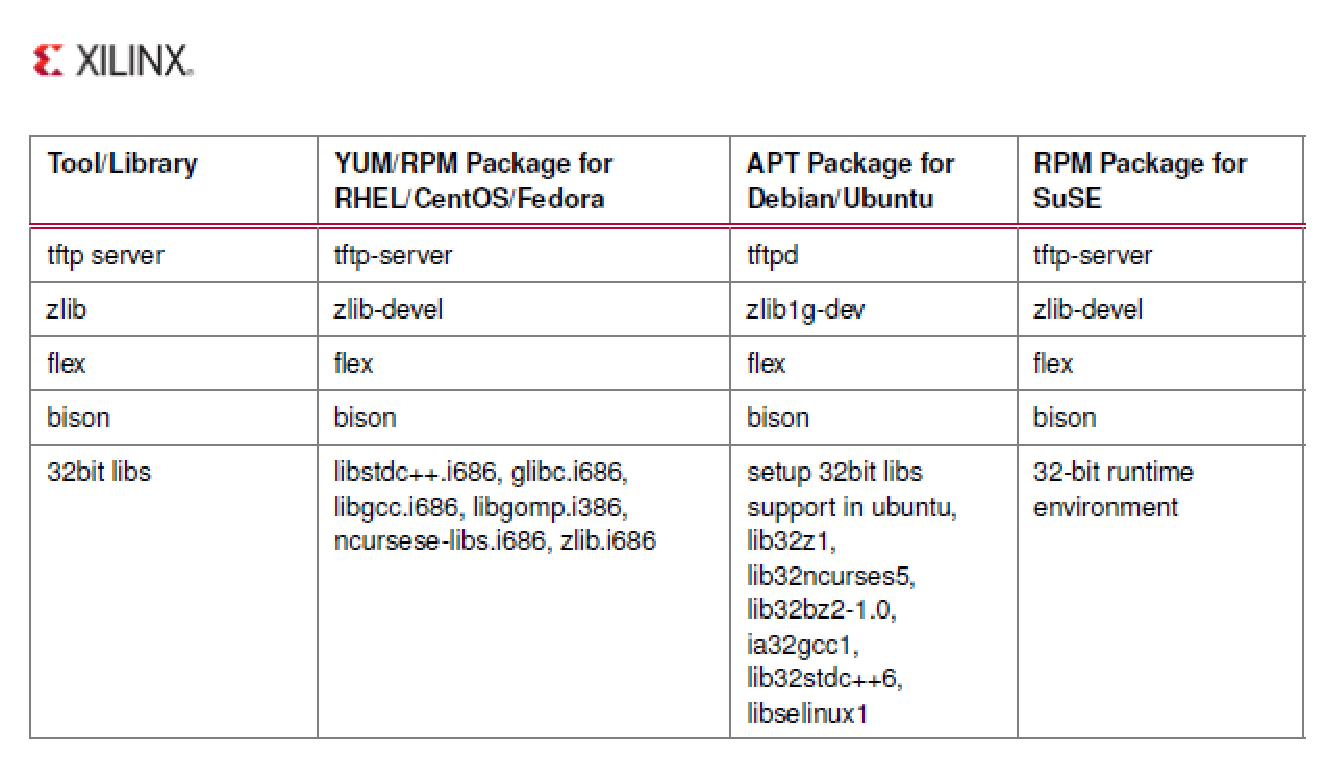
\includegraphics[width=0.85\textwidth]{./images/preinstall_3.eps}
	\caption{Pre-install packcages}
	\label{fig:preinstall_2} 
\end{figure}

\clearpage


Xilinx에서 제공하는 linux image를 생성하는 툴인 peta-linux를 설치하기 위하여 그림 \ref{fig:preinstall_2} 에서와 같이 Debian/Ubuntu에서 언급한 내용을 설치한다. 이는 64bit 환경하에서 petalinux를 설치하기 위한 추가적 32bit용 패키지 모듈이다.

아래 리스트는 상위 그림 \ref{fig:preinstall_2} 에서 언급한 모듈에 대한 설치 내용을 보여준다.


\begin{lstlisting}[style=termstyle]
root@silee:/home/ctrluser# cat typescript 
Script started on Tue 07 Apr 2015 10:23:32 AM KST
root@silee:/home/ctrluser# 
root@silee:/home/ctrluser# aptitude install tofrodos
The following NEW packages will be installed:
tofrodos 
0 packages upgraded, 1 newly installed, 0 to remove and 0 not upgraded.
Need to get 21.9 kB of archives. After unpacking 68.6 kB will be used.
Get: 1 http://ftp.debian.org/debian/ wheezy/main tofrodos amd64 1.7.9.debian.1-1 [21.9 kB]
Fetched 21.9 kB in 2s (8,759 B/s)   
Selecting previously unselected package tofrodos.
(Reading database ... 317356 files and directories currently installed.)
Unpacking tofrodos (from .../tofrodos_1.7.9.debian.1-1_amd64.deb) ...
Processing triggers for man-db ...
Setting up tofrodos (1.7.9.debian.1-1) ...

root@silee:/home/ctrluser# aptitude install iproute gawk git-core
The following NEW packages will be installed:
gawk git-core 
0 packages upgraded, 2 newly installed, 0 to remove and 0 not upgraded.
Need to get 973 kB of archives. After unpacking 2,345 kB will be used.
Get: 1 http://ftp.debian.org/debian/ wheezy/main gawk amd64 1:4.0.1+dfsg-2.1 [972 kB]
Get: 2 http://ftp.debian.org/debian/ wheezy/main git-core all 1:1.7.10.4-1+wheezy1 [1,336B]
Fetched 973 kB in 8s (116 kB/s)
Selecting previously unselected package gawk.
(Reading database ... 317366 files and directories currently installed.)
Unpacking gawk (from .../gawk_1%3a4.0.1+dfsg-2.1_amd64.deb) ...
Selecting previously unselected package git-core.
Unpacking git-core (from .../git-core_1%3a1.7.10.4-1+wheezy1_all.deb) ...
Processing triggers for man-db ...
Setting up gawk (1:4.0.1+dfsg-2.1) ...
Setting up git-core (1:1.7.10.4-1+wheezy1) ...

root@silee:/home/ctrluser# aptitude install net-tools
No packages will be installed, upgraded, or removed.
0 packages upgraded, 0 newly installed, 0 to remove and 0 not upgraded.
Need to get 0 B of archives. After unpacking 0 B will be used.

root@silee:/home/ctrluser# aptitude search net-tools
i   net-tools                - The NET-3 networking toolkit                                       
root@silee:/home/ctrluser# aptitude search ncurses-dev
p   libcunit1-ncurses-dev                   - Unit Testing Library for C (ncurses) -- development files          
p   libghc-ncurses-dev                      - Haskell bindings to the GNU ncurses library                        
v   libghc-ncurses-dev-0.2.1-8df37    		-                                                                    
p   libkaya-ncurses-dev                     - Ncurses binding for kaya                                           
v   libncurses-dev    						-      
v   ncurses-dev       						-
                                                                    
root@silee:/home/ctrluser# aptitude install ncurses-dev
Note: selecting "libncurses5-dev" instead of the
virtual package "ncurses-dev"
The following NEW packages will be installed:
libncurses5-dev 
0 packages upgraded, 1 newly installed, 0 to remove and 0 not upgraded.
Need to get 223 kB of archives. After unpacking 1,032 kB will be used.
Get: 1 http://ftp.debian.org/debian/ wheezy/main libncurses5-dev amd64 5.9-10 [223 kB]
Fetched 223 kB in 3s (59.8 kB/s)          
Selecting previously unselected package libncurses5-dev.
(Reading database ... 317477 files and directories currently installed.)
Unpacking libncurses5-dev (from .../libncurses5-dev_5.9-10_amd64.deb) ...
Setting up libncurses5-dev (5.9-10) ...

root@silee:/home/ctrluser# aptitude search ncurses-dev
p   libcunit1-ncurses-dev                    - Unit Testing Library for C (ncurses) -- development files          
p   libghc-ncurses-dev                       - Haskell bindings to the GNU ncurses library                        
v   libghc-ncurses-dev-0.2.1-8df37           -                                                                    
p   libkaya-ncurses-dev                      - Ncurses binding for kaya                                           
v   libncurses-dev   						 -                                                                    
v   ncurses-dev                              -                                                                 
   
root@silee:/home/ctrluser# aptitude search libncurses5-dev
i   libncurses5-dev                          - developer's libraries for ncurses                                  
root@silee:/home/ctrluser# aptitude install tftpd
The following NEW packages will be installed:
openbsd-inetd{a} tftpd 
0 packages upgraded, 2 newly installed, 0 to remove and 0 not upgraded.
Need to get 55.1 kB of archives. After unpacking 109 kB will be used.
Do you want to continue? [Y/n/?] Y
Get: 1 http://ftp.debian.org/debian/ wheezy/main openbsd-inetd amd64 0.20091229-2 [38.1 kB]
Get: 2 http://ftp.debian.org/debian/ wheezy/main tftpd amd64 0.17-18 [17.0 kB]
Fetched 55.1 kB in 2s (23.4 kB/s)  
Selecting previously unselected package openbsd-inetd.
(Reading database ... 317514 files and directories currently installed.)
Unpacking openbsd-inetd (from .../openbsd-inetd_0.20091229-2_amd64.deb) ...
Selecting previously unselected package tftpd.
Unpacking tftpd (from .../tftpd_0.17-18_amd64.deb) ...
Processing triggers for man-db ...
Setting up openbsd-inetd (0.20091229-2) ...
[ ok ] Stopping internet superserver: inetd.
[info] Not starting internet superserver: no services enabled.
Setting up tftpd (0.17-18) ...

root@silee:/home/ctrluser# aptitude install zlib1g-dev
No packages will be installed, upgraded, or removed.
0 packages upgraded, 0 newly installed, 0 to remove and 0 not upgraded.
Need to get 0 B of archives. After unpacking 0 B will be used.

root@silee:/home/ctrluser# aptitude search zlib1g
i   zlib1g                              - compression library - runtime                                      
p   zlib1g-dbg                          - compression library - development                                  
i A zlib1g-dev                          - compression library - development                                  
root@silee:/home/ctrluser# aptitude search flex
p   cl-flexi-streams                    - Flexi-streams: Flexible bivalent streams for Common Lisp           
p   cl-flexichain                       - An efficient gap buffer with a well-defined external protocol      
p   flex                                - A fast lexical analyzer generator.                                 
p   flex-doc                            - Documentation for flex (a fast lexical analyzer generator).        
p   flex-old                            - Old version of the fast lexical analyzer generator                 
p   flex-old-doc                        - Documentation for an old flex (a fast lexical analyzer generator)  
p   flexbackup                          - Flexible backup tool for small to medium sized installations       
p   flexc++                             - Flex-style scanner generator for C++                               
p   flexloader                          - utility to configure SRAM based ALTERA devices                     
v   flexmem                             -                                                                    
p   flexml                              - Fast validating XML processors and applications generator          
p   jflex                               - lexical analyzer generator for Java                                
p   libdatetime-format-flexible-perl    - Perl module to transform strings into DateTime objects             
p   libflexdock-java                    - Swing Java docking framework                                       
p   libflexdock-java-demo               - Swing Java docking framework - demos and examples                  
p   libflexdock-java-doc                - Swing Java docking framework - demos and examples                  
p   libflexmock-ruby                    - Transitional package for ruby-flexmock                             
p   libflexmock-ruby1.8                 - Transitional package for ruby-flexmock                             
p   libflexmock-ruby1.9.1               - Transitional package for ruby-flexmock                             
p   python-flexmock                     - Mock/Stub/Spy library for Python                                   
p   python3-flexmock                    - Mock/Stub/Spy library for Python 3                                 
p   ruby-flexmock                       - simple and flexible mock objects for testing                       
root@silee:/home/ctrluser# aptitude search flex
p   cl-flexi-streams                    - Flexi-streams: Flexible bivalent streams for Common Lisp           
p   cl-flexichain                       - An efficient gap buffer with a well-defined external protocol      
p   flex                                - A fast lexical analyzer generator.                                 
p   flex-doc                            - Documentation for flex (a fast lexical analyzer generator).        
p   flex-old                            - Old version of the fast lexical analyzer generator                 
p   flex-old-doc                        - Documentation for an old flex (a fast lexical analyzer generator)  
p   flexbackup                          - Flexible backup tool for small to medium sized installations       
p   flexc++                             - Flex-style scanner generator for C++                               
p   flexloader                          - utility to configure SRAM based ALTERA devices                     
v   flexmem                             -                                                                    
p   flexml                              - Fast validating XML processors and applications generator          
p   jflex                               - lexical analyzer generator for Java                                
p   libdatetime-format-flexible-perl    - Perl module to transform strings into DateTime objects             
p   libflexdock-java                    - Swing Java docking framework                                       
p   libflexdock-java-demo               - Swing Java docking framework - demos and examples                  
p   libflexdock-java-doc                - Swing Java docking framework - demos and examples                  
p   libflexmock-ruby                    - Transitional package for ruby-flexmock                             
p   libflexmock-ruby1.8                 - Transitional package for ruby-flexmock                             
p   libflexmock-ruby1.9.1               - Transitional package for ruby-flexmock                             
p   python-flexmock                     - Mock/Stub/Spy library for Python                                   
p   python3-flexmock                    - Mock/Stub/Spy library for Python 3                                 
p   ruby-flexmock                       - simple and flexible mock objects for testing                       
root@silee:/home/ctrluser# aptitude install flex
The following NEW packages will be installed: flex 
0 packages upgraded, 1 newly installed, 0 to remove and 0 not upgraded.
Need to get 332 kB of archives. After unpacking 944 kB will be used.
Get: 1 http://ftp.debian.org/debian/ wheezy/main flex amd64 2.5.35-10.1 [332 kB]
Fetched 332 kB in 4s (71.4 kB/s)
Selecting previously unselected package flex.
(Reading database ... 317530 files and directories currently installed.)
Unpacking flex (from .../flex_2.5.35-10.1_amd64.deb) ...
Processing triggers for install-info ...
Processing triggers for man-db ...
Setting up flex (2.5.35-10.1) ...

root@silee:/home/ctrluser# aptitude install bison
The following NEW packages will be installed:
bison libbison-dev{a} 
0 packages upgraded, 2 newly installed, 0 to remove and 0 not upgraded.
Need to get 977 kB of archives. After unpacking 1,846 kB will be used.
Do you want to continue? [Y/n/?] Y
Get: 1 http://ftp.debian.org/debian/ wheezy/main libbison-dev amd64 1:2.5.dfsg-2.1 [289 kB]
Get: 2 http://ftp.debian.org/debian/ wheezy/main bison amd64 1:2.5.dfsg-2.1 [689 kB]
Fetched 977 kB in 7s (126 kB/s)                                                                                                    
Selecting previously unselected package libbison-dev:amd64.
(Reading database ... 317569 files and directories currently installed.)
Unpacking libbison-dev:amd64 (from .../libbison-dev_1%3a2.5.dfsg-2.1_amd64.deb) ...
Selecting previously unselected package bison.
Unpacking bison (from .../bison_1%3a2.5.dfsg-2.1_amd64.deb) ...
Processing triggers for man-db ...
Setting up libbison-dev:amd64 (1:2.5.dfsg-2.1) ...
Setting up bison (1:2.5.dfsg-2.1) ...
update-alternatives: using /usr/bin/bison.yacc to provide /usr/bin/yacc (yacc) in auto mode

root@silee:/home/ctrluser# aptitude search lib32z1
p   lib32z1                                   - compression library - 32 bit runtime                               
p   lib32z1-dev                               - compression library - 32 bit development                           

root@silee:/home/ctrluser# aptitude install lib32z1
The following NEW packages will be installed:
lib32z1 libc6-i386{a} 
0 packages upgraded, 2 newly installed, 0 to remove and 0 not upgraded.
Need to get 4,111 kB of archives. After unpacking 9,407 kB will be used.
Do you want to continue? [Y/n/?] Y
Get: 1 http://security.debian.org/ wheezy/updates/main libc6-i386 amd64 2.13-38+deb7u8 [4,022 kB]
Get: 2 http://ftp.debian.org/debian/ wheezy/main lib32z1 amd64 1:1.2.7.dfsg-13 [89.0 kB]
Fetched 4,111 kB in 2s (1,444 kB/s)                                    
Selecting previously unselected package libc6-i386.
(Reading database ... 317676 files and directories currently installed.)
Unpacking libc6-i386 (from .../libc6-i386_2.13-38+deb7u8_amd64.deb) ...
Selecting previously unselected package lib32z1.
Unpacking lib32z1 (from .../lib32z1_1%3a1.2.7.dfsg-13_amd64.deb) ...
Setting up libc6-i386 (2.13-38+deb7u8) ...
Setting up lib32z1 (1:1.2.7.dfsg-13) ...

root@silee:/home/ctrluser# aptitude search lib32z1
i   lib32z1                                   - compression library - 32 bit runtime                               
p   lib32z1-dev                               - compression library - 32 bit development                           
root@silee:/home/ctrluser# aptitude search lib32ncurses5
p   lib32ncurses5                             - shared libraries for terminal handling (32-bit)                    
p   lib32ncurses5-dev                         - developer's libraries for ncurses (32-bit)                         
root@silee:/home/ctrluser# aptitude install lib32ncurses5
The following NEW packages will be installed:
lib32ncurses5 lib32tinfo5{a} 
0 packages upgraded, 2 newly installed, 0 to remove and 0 not upgraded.
Need to get 384 kB of archives. After unpacking 688 kB will be used.
Do you want to continue? [Y/n/?] Y
Get: 1 http://ftp.debian.org/debian/ wheezy/main lib32tinfo5 amd64 5.9-10 [268 kB]
Get: 2 http://ftp.debian.org/debian/ wheezy/main lib32ncurses5 amd64 5.9-10 [115 kB]
Fetched 384 kB in 5s (74.4 kB/s)        
Selecting previously unselected package lib32tinfo5.
(Reading database ... 317986 files and directories currently installed.)
Unpacking lib32tinfo5 (from .../lib32tinfo5_5.9-10_amd64.deb) ...
Selecting previously unselected package lib32ncurses5.
Unpacking lib32ncurses5 (from .../lib32ncurses5_5.9-10_amd64.deb) ...
Setting up lib32tinfo5 (5.9-10) ...
Setting up lib32ncurses5 (5.9-10) ...

root@silee:/home/ctrluser# aptitude install lib32bz2
Couldn't find package "lib32bz2".  However, the following
packages contain "lib32bz2" in their name:
lib32bz2-1.0 lib32bz2-dev 
Couldn't find package "lib32bz2".  However, the following
packages contain "lib32bz2" in their name:
lib32bz2-1.0 lib32bz2-dev 
No packages will be installed, upgraded, or removed.
0 packages upgraded, 0 newly installed, 0 to remove and 0 not upgraded.
Need to get 0 B of archives. After unpacking 0 B will be used.

root@silee:/home/ctrluser# aptitude search lib32bz2
p   lib32bz2-1.0                              - high-quality block-sorting file compressor library - 32bit runtime 
p   lib32bz2-dev                              - high-quality block-sorting file compressor library - 32bit developm
root@silee:/home/ctrluser# aptitude install lib32bz2-1.0
The following NEW packages will be installed: lib32bz2-1.0 
0 packages upgraded, 1 newly installed, 0 to remove and 0 not upgraded.
Need to get 40.5 kB of archives. After unpacking 77.8 kB will be used.
Get: 1 http://ftp.debian.org/debian/ wheezy/main lib32bz2-1.0 amd64 1.0.6-4 [40.5 kB]
Fetched 40.5 kB in 1s (21.3 kB/s)       
Selecting previously unselected package lib32bz2-1.0.
(Reading database ... 318003 files and directories currently installed.)
Unpacking lib32bz2-1.0 (from .../lib32bz2-1.0_1.0.6-4_amd64.deb) ...
Setting up lib32bz2-1.0 (1.0.6-4) ...

root@silee:/home/ctrluser# aptitude search lib32gcc
p   lib32gcc1                                 - GCC support library (32 bit Version)                               
p   lib32gcc1-dbg                             - GCC support library (debug symbols)                                
root@silee:/home/ctrluser# aptitude search lib32stdc++
p   lib32stdc++6                              - GNU Standard C++ Library v3 (32 bit Version)                       
p   lib32stdc++6-4.4-dbg                      - GNU Standard C++ Library v3 (debugging files)                      
p   lib32stdc++6-4.6-dbg                      - GNU Standard C++ Library v3 (debugging files)                      
p   lib32stdc++6-4.7-dbg                      - GNU Standard C++ Library v3 (debugging files)                      
root@silee:/home/ctrluser# aptitude install lib32stdc++6
The following NEW packages will be installed:
lib32gcc1{a} lib32stdc++6 
0 packages upgraded, 2 newly installed, 0 to remove and 0 not upgraded.
Need to get 400 kB of archives. After unpacking 1,336 kB will be used.
Do you want to continue? [Y/n/?] Y
Get: 1 http://ftp.debian.org/debian/ wheezy/main lib32gcc1 amd64 1:4.7.2-5 [53.2 kB]
Get: 2 http://ftp.debian.org/debian/ wheezy/main lib32stdc++6 amd64 4.7.2-5 [346 kB]
Fetched 400 kB in 5s (70.3 kB/s)       
Selecting previously unselected package lib32gcc1.
(Reading database ... 318009 files and directories currently installed.)
Unpacking lib32gcc1 (from .../lib32gcc1_1%3a4.7.2-5_amd64.deb) ...
Selecting previously unselected package lib32stdc++6.
Unpacking lib32stdc++6 (from .../lib32stdc++6_4.7.2-5_amd64.deb) ...
Setting up lib32gcc1 (1:4.7.2-5) ...
Setting up lib32stdc++6 (4.7.2-5) ...

root@silee:/home/ctrluser# aptitude search libselinux1
i   libselinux1                               - SELinux runtime shared libraries                                   
p   libselinux1-dev                           - SELinux development headers                                        
root@silee:/home/ctrluser# aptitude search libgtk2.0
i A libgtk2.0-0                               - GTK+ graphical user interface library                              
p   libgtk2.0-0-dbg                           - GTK+ libraries and debugging symbols                               
i A libgtk2.0-bin                             - programs for the GTK+ graphical user interface library             
i A libgtk2.0-cil                             - CLI binding for the GTK+ toolkit 2.12                              
p   libgtk2.0-cil-dev                         - CLI binding for the GTK+ toolkit 2.12                              
i A libgtk2.0-common                          - common files for the GTK+ graphical user interface library         
p   libgtk2.0-dev                             - development files for the GTK+ library                             
p   libgtk2.0-doc                             - documentation for the GTK+ graphical user interface library        
root@silee:/home/ctrluser# aptitude search libgtk2.0:i386
root@silee:/home/ctrluser# aptitude search libgtk2.0-0
i A libgtk2.0-0                               - GTK+ graphical user interface library                              
p   libgtk2.0-0-dbg                           - GTK+ libraries and debugging symbols                               
root@silee:/home/ctrluser# aptitude search libgtk2.0-0:i386
root@silee:/home/ctrluser# aptitude search libncurse
v   libncurses-dev                            -                                                                    
p   libncurses-gst                            - Ncurses bindings for GNU Smalltalk                                 
p   libncurses-ruby                           - Transitional package for ruby-ncurses                              
p   libncurses-ruby1.8                        - Transitional package for ruby-ncurses                              
p   libncurses-ruby1.9                        - Transitional package for ruby-ncurses                              
p   libncurses-ruby1.9.1                      - Transitional package for ruby-ncurses                              
i   libncurses5                               - shared libraries for terminal handling                             
p   libncurses5-dbg                           - debugging/profiling libraries for ncurses                          
i   libncurses5-dev                           - developer's libraries for ncurses                                  
p   libncursesada-dbg                         - Ada binding to the ncurses text interface library: debug symbols   
p   libncursesada-doc                         - Ada binding to the ncurses text interface library: documentation   
p   libncursesada2                            - Ada binding to the ncurses text interface library: shared library  
p   libncursesada2-dev                        - Ada binding to the ncurses text interface library: development     
i   libncursesw5                              - shared libraries for terminal handling (wide character support)    
p   libncursesw5-dbg                          - debugging/profiling libraries for ncursesw                         
p   libncursesw5-dev                          - developer's libraries for ncursesw                                 
root@silee:/home/ctrluser# aptitude install libncursesw5-dev
The following NEW packages will be installed:
libncursesw5-dev 
0 packages upgraded, 1 newly installed, 0 to remove and 0 not upgraded.
Need to get 257 kB of archives. After unpacking 1,160 kB will be used.
Get: 1 http://ftp.debian.org/debian/ wheezy/main libncursesw5-dev amd64 5.9-10 [257 kB]
Fetched 257 kB in 4s (53.8 kB/s)           
Selecting previously unselected package libncursesw5-dev.
(Reading database ... 318014 files and directories currently installed.)
Unpacking libncursesw5-dev (from .../libncursesw5-dev_5.9-10_amd64.deb) ...
Setting up libncursesw5-dev (5.9-10) ...

root@silee:/home/ctrluser# aptitude search i386
p   bootcd-i386                                  - bootcd extension to create images that can boot on i386            
p   debian-installer-7.0-netboot-i386            - Debian-installer network boot images for i386                      
p   debian-installer-7.0-netboot-kfreebsd-i386   - Debian-installer network boot images for kfreebsd-i386             
v   debian-installer-netboot-i386                -                                                                    
v   debian-installer-netboot-kfreebsd-i386       -                                                                    
p   installation-guide-i386                      - Debian installation guide for i386                                 
p   installation-guide-kfreebsd-i386             - Debian installation guide for kFreeBSD i386                        
p   libc6-dev-i386                               - Embedded GNU C Library: 32-bit development libraries for AMD64     
i A libc6-i386                                   - Embedded GNU C Library: 32-bit shared libraries for AMD64          
root@silee:/home/ctrluser# aptitude install libc6-dev-i386
The following NEW packages will be installed:
gcc-4.7-multilib{a} gcc-multilib{a} lib32gomp1{a} lib32itm1{a} lib32quadmath0{a} libc6-dev-i386 
0 packages upgraded, 6 newly installed, 0 to remove and 0 not upgraded.
Need to get 4,433 kB of archives. After unpacking 10.5 MB will be used.
Do you want to continue? [Y/n/?] Y
Get: 1 http://ftp.debian.org/debian/ wheezy/main lib32gomp1 amd64 4.7.2-5 [29.9 kB]
Get: 2 http://ftp.debian.org/debian/ wheezy/main lib32itm1 amd64 4.7.2-5 [35.8 kB]
Get: 3 http://security.debian.org/ wheezy/updates/main libc6-dev-i386 amd64 2.13-38+deb7u8 [1,593 kB]
Get: 4 http://ftp.debian.org/debian/ wheezy/main lib32quadmath0 amd64 4.7.2-5 [198 kB]
Get: 5 http://ftp.debian.org/debian/ wheezy/main gcc-4.7-multilib amd64 4.7.2-5 [2,576 kB]
Get: 6 http://ftp.debian.org/debian/ wheezy/main gcc-multilib amd64 4:4.7.2-1 [894 B]
Fetched 4,433 kB in 13s (327 kB/s)
Selecting previously unselected package libc6-dev-i386.
(Reading database ... 318050 files and directories currently installed.)
Unpacking libc6-dev-i386 (from .../libc6-dev-i386_2.13-38+deb7u8_amd64.deb) ...
Selecting previously unselected package lib32gomp1.
Unpacking lib32gomp1 (from .../lib32gomp1_4.7.2-5_amd64.deb) ...
Selecting previously unselected package lib32itm1.
Unpacking lib32itm1 (from .../lib32itm1_4.7.2-5_amd64.deb) ...
Selecting previously unselected package lib32quadmath0.
Unpacking lib32quadmath0 (from .../lib32quadmath0_4.7.2-5_amd64.deb) ...
Selecting previously unselected package gcc-4.7-multilib.
Unpacking gcc-4.7-multilib (from .../gcc-4.7-multilib_4.7.2-5_amd64.deb) ...
Selecting previously unselected package gcc-multilib.
Unpacking gcc-multilib (from .../gcc-multilib_4%3a4.7.2-1_amd64.deb) ...
Setting up libc6-dev-i386 (2.13-38+deb7u8) ...
Setting up lib32gomp1 (4.7.2-5) ...
Setting up lib32itm1 (4.7.2-5) ...
Setting up lib32quadmath0 (4.7.2-5) ...
Setting up gcc-4.7-multilib (4.7.2-5) ...
Setting up gcc-multilib (4:4.7.2-1) ...
\end{lstlisting}

아래 Xilinx 다운로드 사이트에서 아래 리스트에 해당하는 software 패키지를 다운받는다. 다운 받은 패키지는 petalinux 설치 메뉴얼에 따라 설치한다.

\begin{lstlisting}[style=termstyle]
http://www.xilinx.com/support/download/index.html/content/xilinx/en/downloadNav/petalinux.html
\end{lstlisting}


\begin{itemize}
	\item Petalinux-v2014.4-final
	\item Avnet-Digilent-ZedBoard-v2014.4-final.bsp
	\item Xilinx Vivado SDK Lin 2014.4.1119-1.tar.gz
\end{itemize}

해당 Petalinux 설치가 완료 되었으면, petalinux command를 사용하여 아래 항목 처럼 project를 생성하고, Xilinkxd에서 제공하는 Zedboard 용 BSP를 사용하여 생성한다.

\begin{lstlisting}[style=termstyle]
ctrluser@silee:~/Petalinux/training/buildBootImage/$ petalinux-create -t project -s /opt/pkg/Avnet-Digilent-ZedBoard-v2014.4-final.bsp
 
ctrluser@silee:~/Petalinux/training/buildBootImage/Avnet-Digilent-ZedBoard-2014.4$ petalinux-build 

INFO: Checking component...
INFO: Generating make files and build linux
INFO: Generating make files for the subcomponents of linux
INFO: Building linux
[ERROR] make: *** linux-kernel: No such file or directory.  Stop.
ERROR: Failed to build linux
\end{lstlisting}

Build시 상위와 같은 error가 발생시 아래 그림 처럼 설정을 변경 후 재빌드한다.

\clearpage
\begin{figure}[h!]
	\centering
	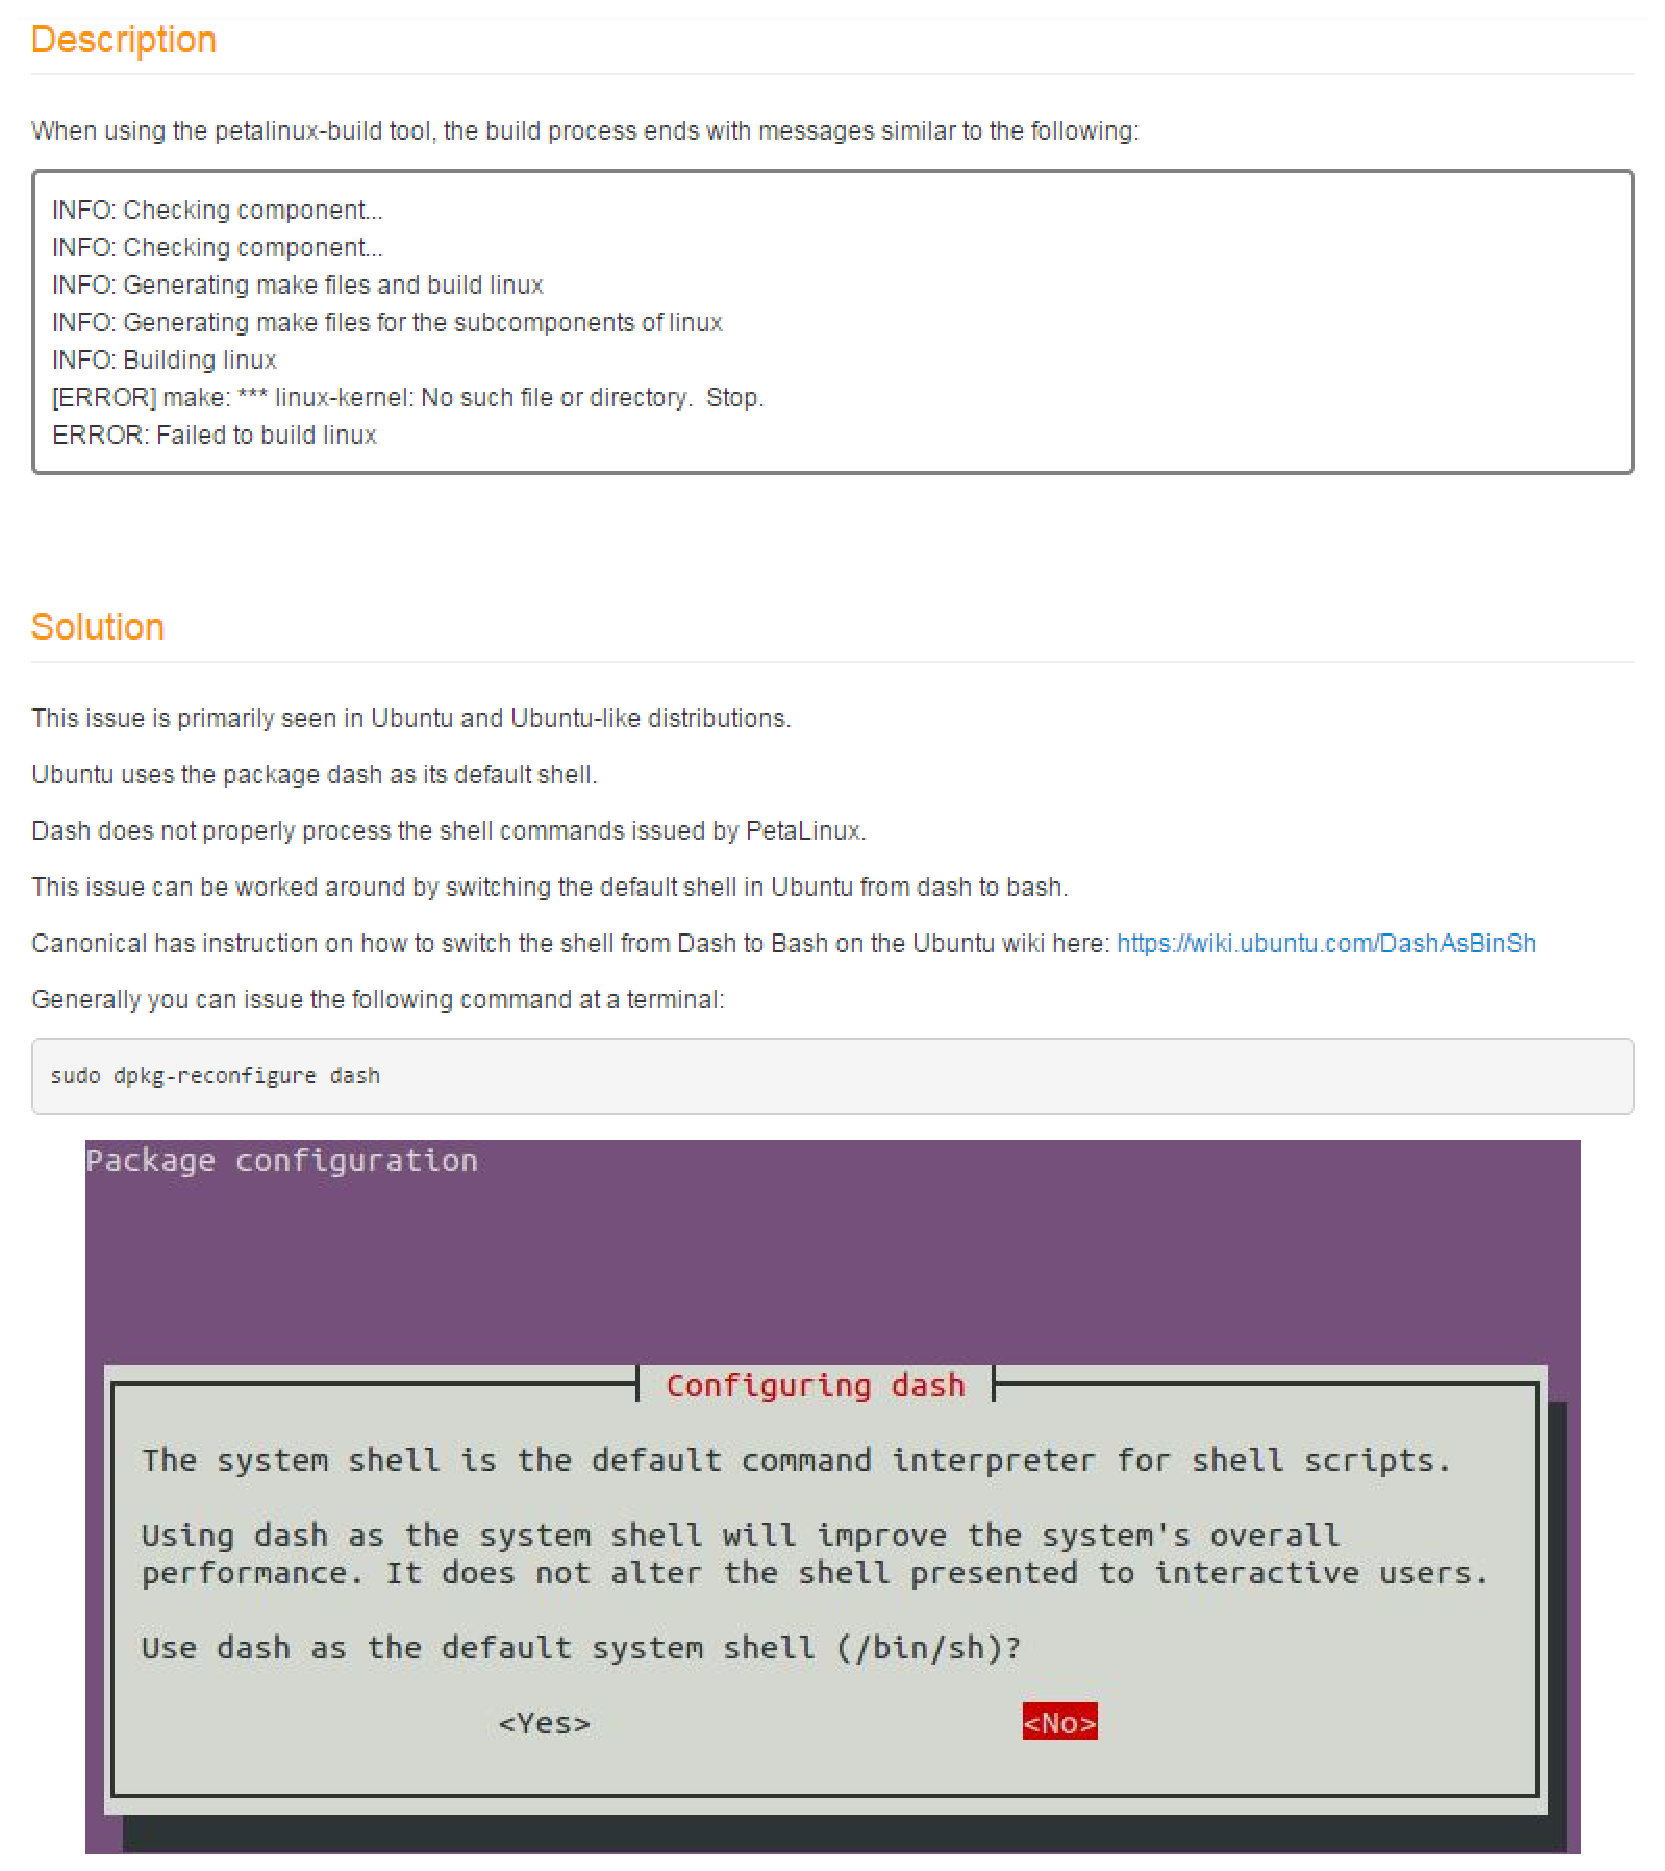
\includegraphics[width=0.85\textwidth]{./images/petalinux-build_error_solve.eps}
	\caption{Build Error}
	\label{fig:build_error} 
\end{figure}

재빌드시 아래와 같은 error 나는 상황이 발생하면 이는 처음 petalinux 설치전 설치하였던 패키지 중 libselinux1에 대한 모듈이 32bit용 모듈이 없기 때문이다.

\begin{lstlisting}[style=termstyle]
ctrluser@silee:~/Petalinux/training/buildBootImage/Avnet-Digilent-ZedBoard-2014.4$ petalinux-build 
INFO: Checking component...
INFO: Generating make files and build linux
INFO: Generating make files for the subcomponents of linux
INFO: Building linux
[INFO ] pre-build linux/rootfs/fwupgrade
[INFO ] pre-build linux/rootfs/peekpoke
[INFO ] pre-build linux/rootfs/uWeb
[INFO ] build linux/kernel
[INFO ] update linux/u-boot source
[INFO ] generate linux/u-boot configuration files
[INFO ] build linux/u-boot
[INFO ] build zynq_fsbl
[INFO ] Expanding stagefs
[ERROR] E: Sub-process /opt/pkg/petalinux-v2014.4-final/tools/packagemanager/bin/dpkg returned an error code (127)
[ERROR] make[2]: *** [.pkg_stagefs] Error 255
[ERROR] make[1]: *** [sub_build_component_/none/packages-repo/single/plnx-repo] Error 2
ERROR: Failed to build linux
\end{lstlisting}

이 문제를 해결하기 위하여는 32bit에서 설치된 libselinux.so.1 라이브러리를 64bit가 설치된 /lib32에 복사를 해주어야 한다.
또는 아래에서 build된 library를 다운 받는다. 안정적인 사용을 위하여는 Debian-32bit 시스템에서 복사해 오기 권장한다.

\begin{lstlisting}[style=termstyle]
http://forums.xilinx.com/t5/Embedded-Linux/2014-2-Image-Build-Processes-Error/td-p/476862/page/3
\end{lstlisting}

\begin{lstlisting}[style=termstyle]
ctrluser@silee:~/Petalinux/training/buildBootImage/Avnet-Digilent-ZedBoard-2014.4$ petalinux-build 
INFO: Checking component...
INFO: Generating make files and build linux
INFO: Generating make files for the subcomponents of linux
INFO: Building linux
[INFO ] pre-build linux/rootfs/fwupgrade
[INFO ] pre-build linux/rootfs/peekpoke
[INFO ] pre-build linux/rootfs/uWeb
[INFO ] build linux/kernel
[INFO ] update linux/u-boot source
[INFO ] generate linux/u-boot configuration files
[INFO ] build linux/u-boot
[INFO ] build zynq_fsbl
[INFO ] build linux/rootfs/fwupgrade
[INFO ] build linux/rootfs/peekpoke
[INFO ] build linux/rootfs/uWeb
[INFO ] build kernel in-tree modules
[INFO ] modules linux/kernel
[INFO ] post-build linux/rootfs/fwupgrade
[INFO ] post-build linux/rootfs/peekpoke
[INFO ] post-build linux/rootfs/uWeb
[INFO ] pre-install linux/rootfs/fwupgrade
[INFO ] pre-install linux/rootfs/peekpoke
[INFO ] pre-install linux/rootfs/uWeb
[INFO ] install system.dtb
[INFO ] install linux/kernel
[INFO ] update linux/u-boot source
[INFO ] generate linux/u-boot configuration files
[INFO ] build linux/u-boot
[INFO ] install linux/u-boot
[INFO ] install sys_init
[INFO ] install linux/rootfs/fwupgrade
[INFO ] install linux/rootfs/peekpoke
[INFO ] install linux/rootfs/uWeb
[INFO ] install kernel in-tree modules
[INFO ] modules_install linux/kernel
[INFO ] post-install linux/rootfs/fwupgrade
[INFO ] post-install linux/rootfs/peekpoke
[INFO ] post-install linux/rootfs/uWeb
[INFO ] package rootfs.cpio to /home/ctrluser/Petalinux/training/buildBootImage/Avnet-Digilent-ZedBoard-2014.4/images/linux
[INFO ] Update and install vmlinux image
[INFO ] vmlinux linux/kernel
[INFO ] install linux/kernel
[INFO ] package zImage
[INFO ] zImage linux/kernel
[INFO ] install linux/kernel
\end{lstlisting}

무사히 빌드가 완료 되었으면 아래 경로에 해당 linux 이미지가 생성됨을 확인한다. 해당 이미지를 확인 할 수 있다면 petalinux 툴 구성이 완료됨을 말한다.

\begin{lstlisting}[style=termstyle]
ctrluser@silee:~/Petalinux/training/buildBootImage/Avnet-Digilent-ZedBoard-2014.4/images/linux$ ls
image.elf  rootfs.cpio     system.dtb        u-boot.bin  u-boot-s.bin  u-boot.srec    urootfs.cpio.gz  zImage
image.ub   rootfs.cpio.gz  System.map.linux  u-boot.elf  u-boot-s.elf  u-boot-s.srec  vmlinux          zynq_fsbl.elf
\end{lstlisting}

\hfil\break
\chapter{Zynq}

\section{특성}

\begin{figure}[h!]
	\centering
	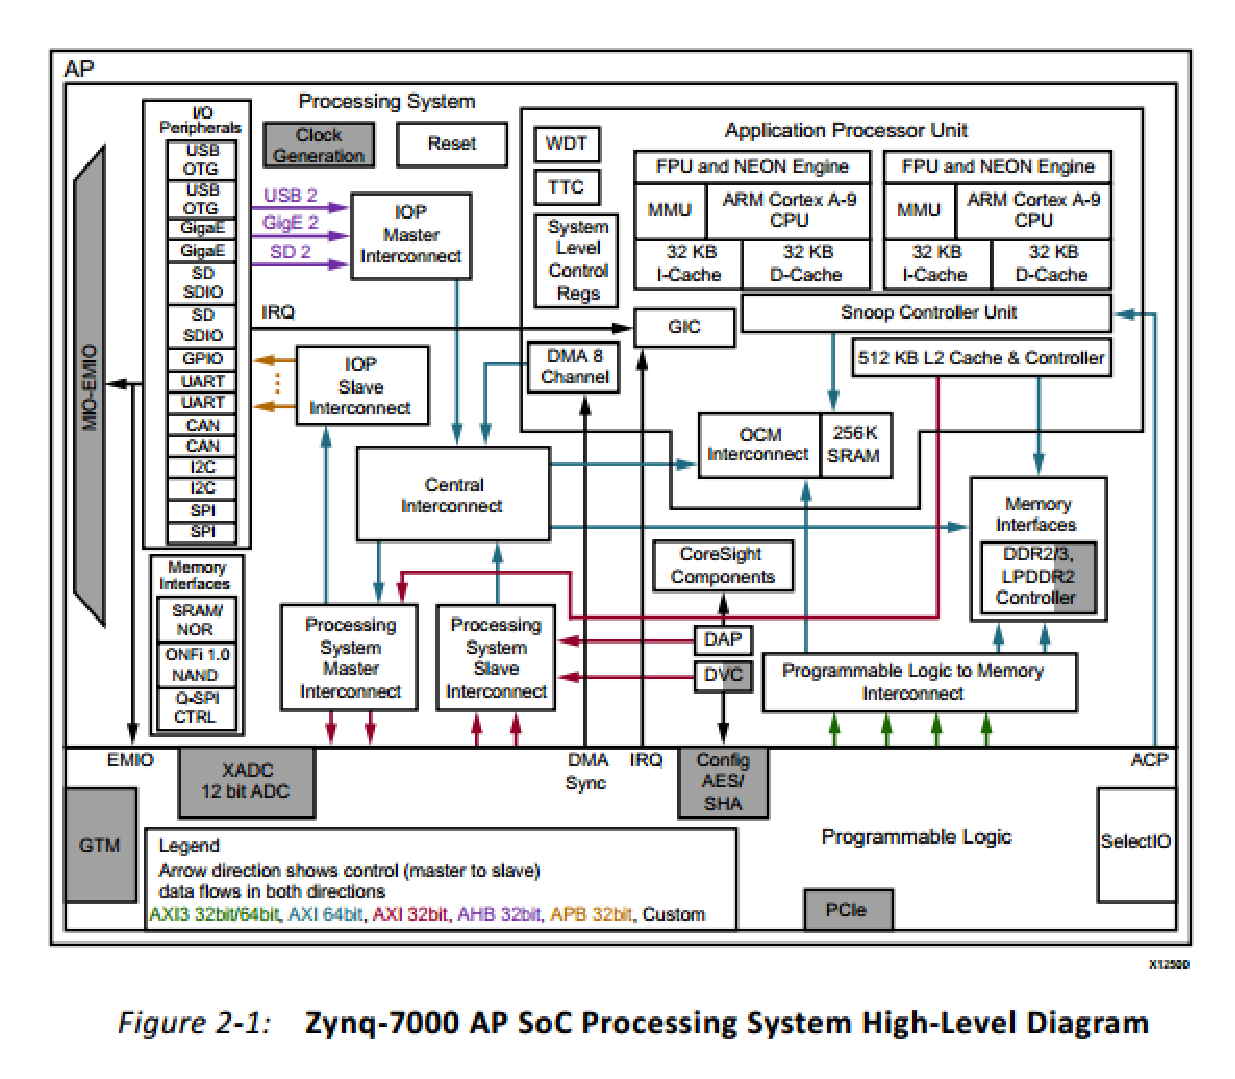
\includegraphics[width=0.95\textwidth, height=0.8\textwidth]{./images/zynq_arch.eps}
	\caption{Zynq Architecture}
	\label{fig:zynq_arch} 
\end{figure}


\clearpage

\bibliographystyle{unsrtnat}
\bibliography{./refs}

\end{document}

